% !TEX root = ../0_main/00_main.tex
\section{Results and Discussion}

\subsection{original Tainter dynamics}

\paragraph{Exemplary development of a tainter inspired society}

\begin{figure}[htb]
    \centering
    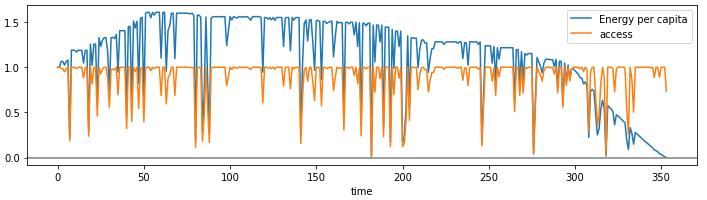
\includegraphics[width=\linewidth]{../figures/network_dev_noexplore.png}
    \caption{Example of development of a society without capacity of exploration (i.e. random change from work to adminstration and vice versa). }
    \label{fig:baseNetworkDev}
\end{figure}


\paragraph{Interplay between network characteristics. Conditions for a beneficial administration}

Find out realistic ranges of efficiency and link density in simplistic societies, in order to be able to discuss the graphic


\begin{figure}[htb]
    \centering
    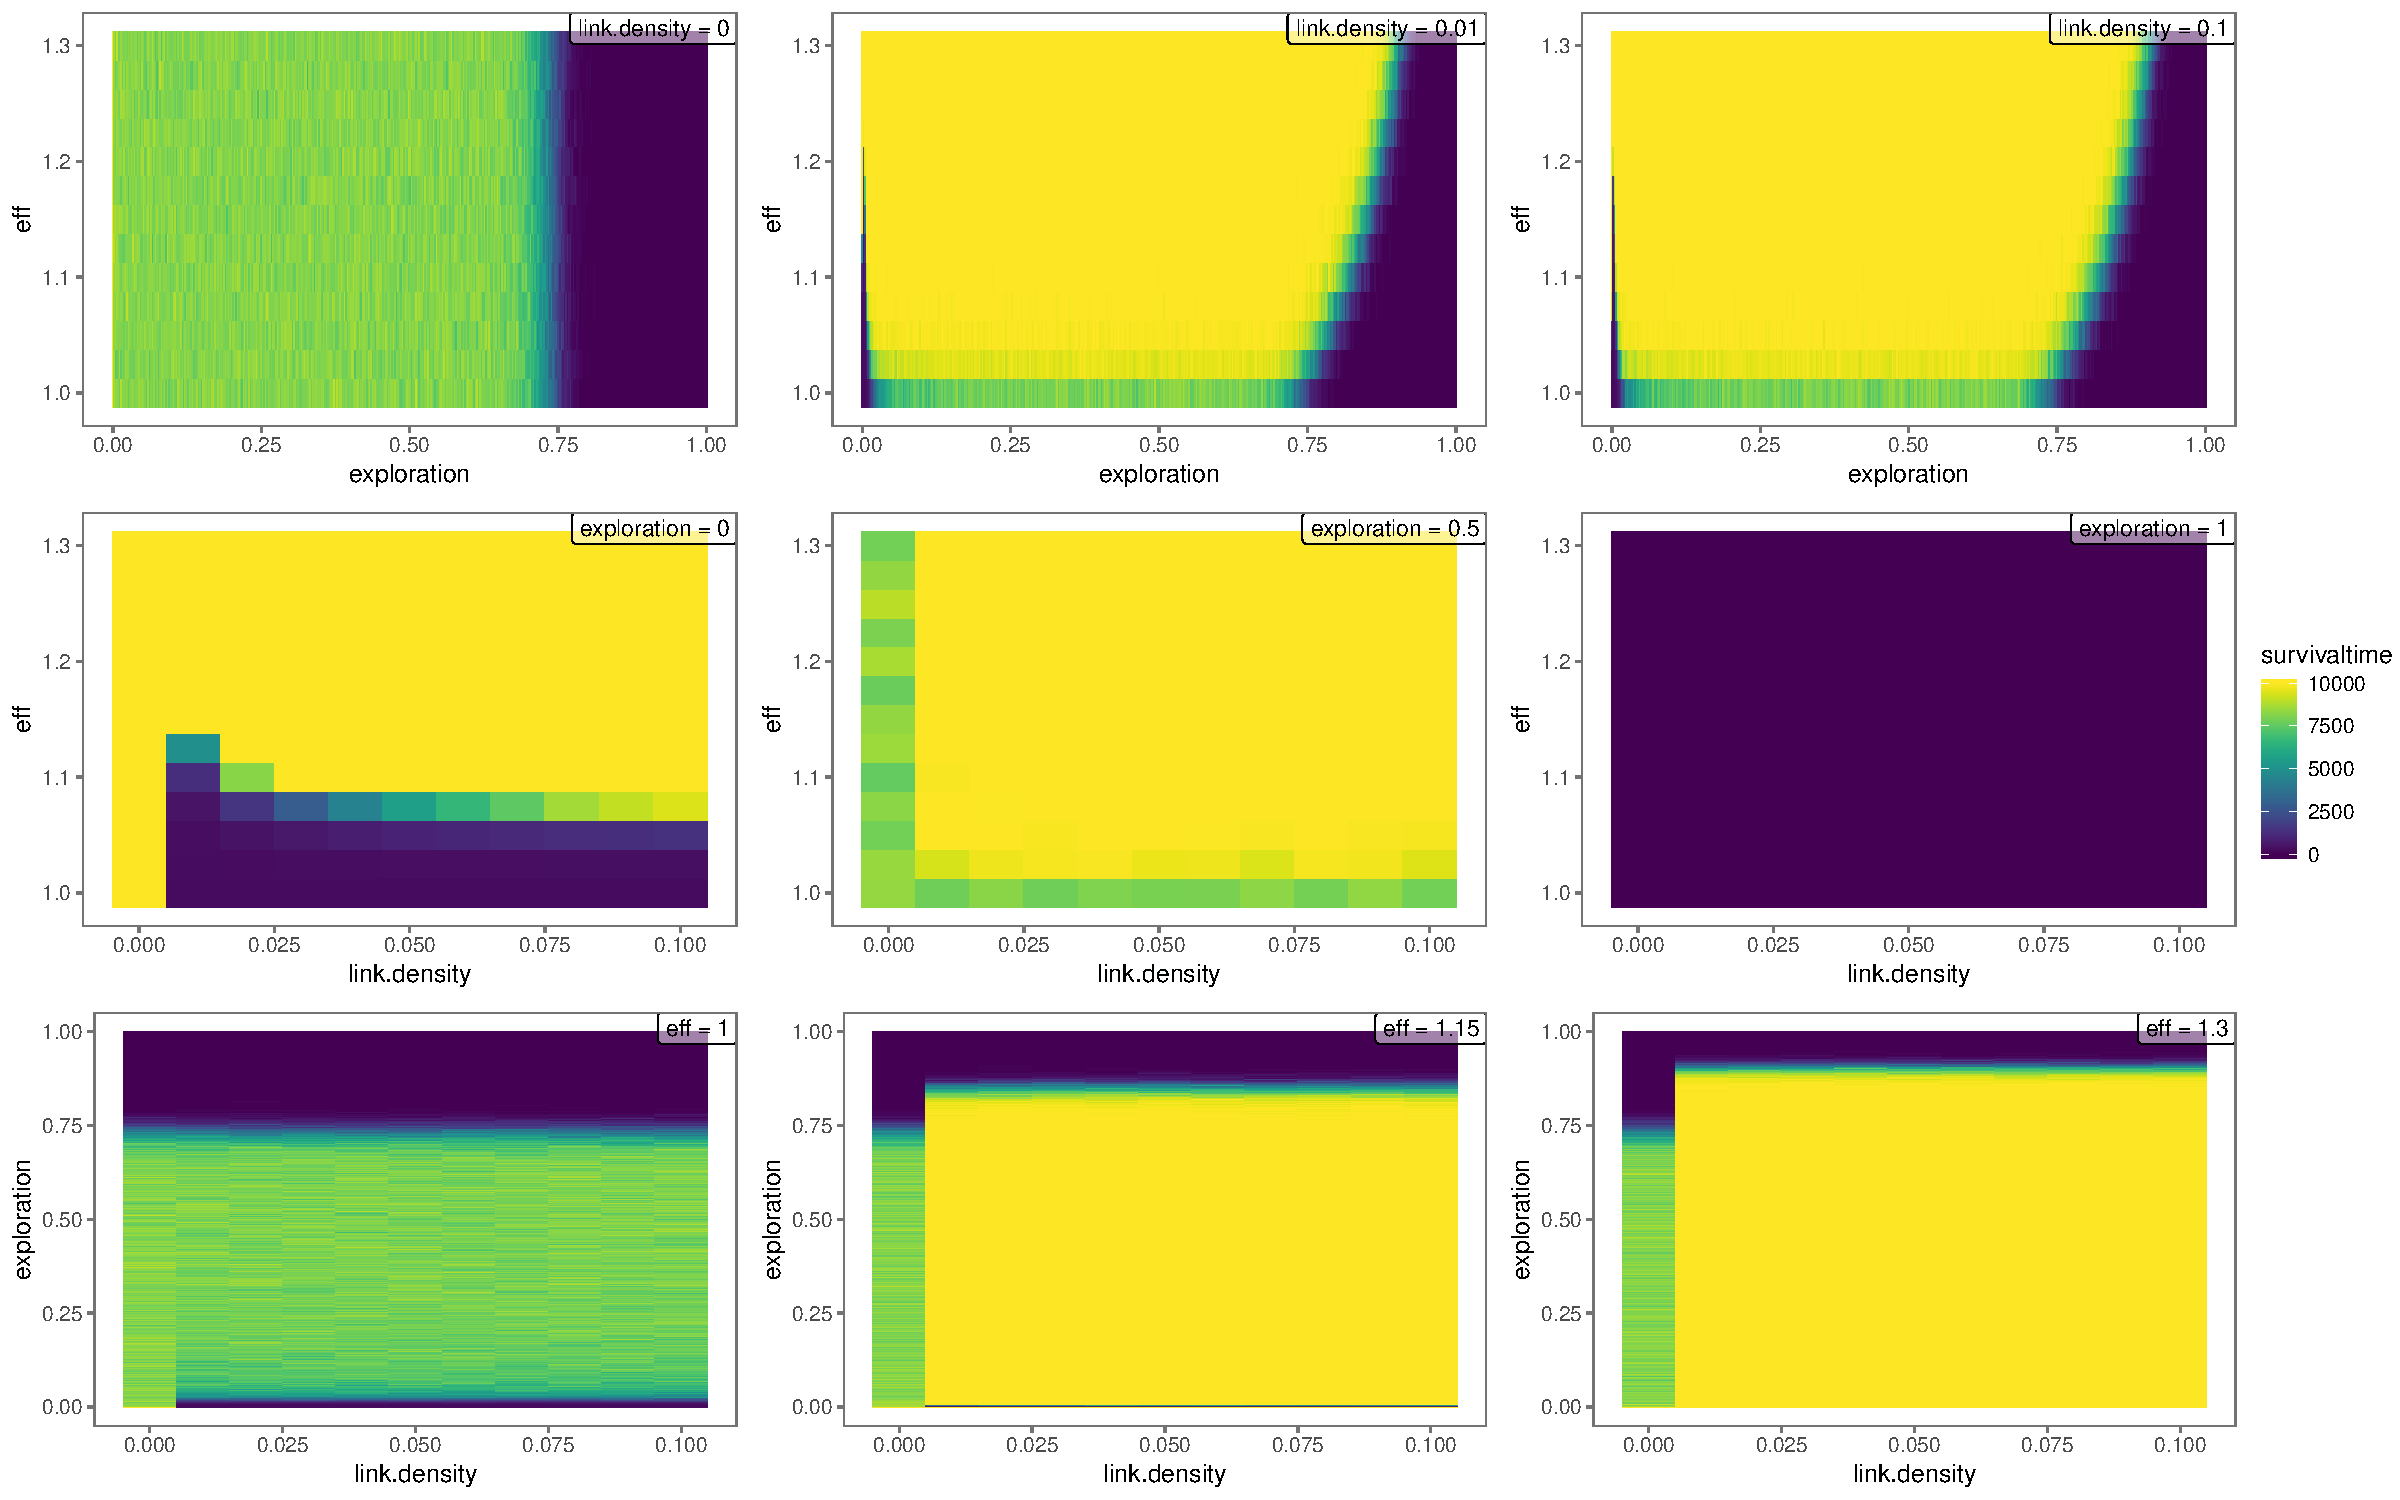
\includegraphics[width = \linewidth]{../figures/survivaltime.pdf}
    \caption{Survival of a network with N = 400 as a function of exploration, link density and efficiency.}
    \label{fig:survival}
\end{figure}


\paragraph{Macroscopic approximation of original Tainter Dynamics}

P_e = 0 in order to leave out exploration term

\subsection{modified Tainter dynamics. Exploration}

\paragraph{model run description}

\paragraph{Low exploration results in highly increased survival times}

\paragraph{extension of macroscopic approximation}
